%% The first command in your LaTeX source must be the \documentclass command.
%%
%% Options:
%% twocolumn : Two column layout.
%% hf: enable header and footer.
\documentclass[
% twocolumn, % Uncomment for two-column layout
% hf,
]{ceurart}

%%
%% One can fix some overfulls
\sloppy
% \usepackage{xmpincl}
\usepackage[utf8]{inputenc}
\usepackage{graphicx}
\usepackage{amsmath, amssymb}
\usepackage{hyperref}
\usepackage{caption}
\usepackage{subcaption}
% \usepackage{cite}
% \usepackage[backend=biber,style=authoryear]{biblatex} 
% \addbibresource{references.bib} 
\usepackage{listings}
\usepackage[numbers]{natbib}
\bibliographystyle{unsrtnat}  % Ensures numerical order of citations
%% auto break lines
\lstset{breaklines=true}
\usepackage{placeins} 

%%
%% end of the preamble, start of the body of the document source.
\begin{document}

%%
%% Rights management information.
%% CC-BY is default license.
\copyrightyear{2025}
\copyrightclause{Copyright for this paper by its authors.
Use permitted under Creative Commons License Attribution 4.0
International (CC BY 4.0).}

%%
%% This command is for the conference information
\conference{Defactify 4: Multimodal Fact-Checking and AI-Generated Image Detection, co-located with  AAAI 2025. 2025. Philadelphia, Pennsylvania, USA  }

%%
%% The "title" command
\title{A Comprehensive Dataset for Human vs. AI Generated Text Detection}

% \tnotemark[1]
% \tnotetext[1]{This document is based on the CEUR-WS template and incorporates topics inspired by the Defactify workshop series.}

\author[1]{Rajarshi Roy}[email=royrajarshi0123@gmail.com]
\author[2]{Nasrin Imanpour}[email=imanpour@email.sc.edu]
\author[3]{Ashhar Aziz}[email=ashhar21137@iiitd.ac.in]
\author[4]{Shashwat Bajpai}[email=f20213041@hyderabad.bits-pilani.ac.in]
\author[5]{Gurpreet Singh}[email=gurpreet.singh@email.com]
\author[6]{Shwetangshu Biswas}[email=shwetangshu.biswas@email.com]
\author[7]{Kapil Wanaskar}[email=kapilw25@gmail.com]
\author[8]{Parth Patwa}[email=parthpatwa@g.ucla.edu]
\author[9]{Subhankar Ghosh}[email=subhankar.ghosh@email.com]
\author[10]{Shreyas Dixit}[email=shreyasrd31@gmail.com]
\author[1]{Nilesh Ranjan Pal}[email=nileshpal530@gmail.com]
\author[2]{Vipula Rawte}[email=vipula.rawte@email.com]
\author[2]{Ritvik Garimella}[email=ritvik.garimella@email.com]
\author[13]{Amitava Das}[email=amitava.das2@wipro.com]
\author[2]{Amit Sheth}[email=amit@sc.edu]
\author[11]{Vasu Sharma}[email=sharma.vasu55@gmail.com]
\author[12]{Aishwarya Naresh Reganti}[email=aish.nr@gmail.com]
\author[11]{Vinija Jain}[email=hi@vinija.ai]
\author[12]{Aman Chadha}[email=hi@amanchadha.com]

\address[1]{Kalyani Government Engineering College, India}
\address[2]{AI Institute University of South Carolina, USA}
\address[3]{IIIT Delhi, India}
\address[4]{BITS Pilani Hyderabad Campus, India}
\address[5]{IIIT Guwahati, India}
\address[6]{National Institute of Technology Silchar, India}
\address[7]{San Jose State University, USA}
\address[8]{University of California Los Angeles, USA}
\address[9]{Washington State University, USA}
\address[10]{Vishwakarma Institute of Information Technology, India}
\address[11]{Meta AI, USA}
\address[12]{Amazon AI, USA}
\address[13]{BITS Pilani, Goa}



\input{abstract}

%%
%% Keywords. The author(s) should pick words that accurately describe
%% the work being presented. Separate the keywords with commas.
\begin{keywords}

\end{keywords}

%%
%% This command processes the author and affiliation and title
%% information and builds the first part of the formatted document.
\maketitle


\section{Introduction}

The recent surge in the capabilities of large language models (LLMs) has dramatically transformed the landscape of text generation. State-of-the-art AI systems can now produce highly coherent and contextually relevant narratives, reports, and articles that are increasingly difficult to distinguish from human-written content. While these advances unlock significant opportunities for innovation across domains such as journalism, education, and digital assistants, they also intensify concerns regarding authenticity, misinformation, and the potential misuse of synthetic text.

The problem of online fake new \cite{}, especially related to elections and diseases \cite{} is exacerbated by AI generated fake news. 

Amidst this evolving environment, the challenge of reliably detecting and attributing AI-generated text has become a research priority \cite{zellers2020defendingneuralfakenews,mitchell2023detectgptzeroshotmachinegeneratedtext}. The capability to differentiate between human-authored and machine-generated content is crucial for safeguarding the integrity of news media, academic publishing, and online discourse. However, progress in this area has been hindered by the scarcity of large, diverse, and well-annotated datasets that contain both human and AI-generated texts under realistic, real-world conditions.

In this paper, we introduce a dataset to detect AI generated text. The dataset is a comprehensive, extensively annotated resource curated to advance research on the detection of AI-generated content. Our dataset is built upon a large-scale collection of authentic news articles from the New York Times, spanning over two decades and covering a broad spectrum of topics. For each sampled article, we provide both the original human-authored narrative and multiple synthetic counterparts generated by leading LLMs, including Gemma-2-9b \cite{gemmateam2024gemma2improvingopen}, Mistral-7B\cite{jiang2023mistral7b}, Qwen-2-72B\cite{bai2023qwentechnicalreport}, LLaMA-8B \cite{touvron2023llamaopenefficientfoundation}, Yi-Large\cite{ai2025yiopenfoundationmodels}, and GPT-4-o\cite{openai2024gpt4technicalreport}. Each sample is enriched with detailed metadata, facilitating nuanced analysis and enabling a wide range of research applications.

The unique structure of the dataset supports tasks such as binary classification (distinguishing human from AI content) and model attribution (identifying the specific LLM responsible for a synthetic text). By bridging the gap between real-world journalistic data and diverse state-of-the-art generative models, our work lays the foundation for more robust benchmarks, and tools that are urgently needed to maintain trust, clarity, and accountability in the age of generative AI.


\section{Related Work}

The rapid advancement of large language models (LLMs) has dramatically increased the quality and prevalence of AI-generated text, making it increasingly difficult to distinguish from human-authored content. This challenge has spurred significant research in two interconnected domains: detecting AI-generated text and identifying fake news and misinformation. Both areas require large-scale, diverse, and well-annotated datasets to develop robust detection methods. In this section, we survey existing datasets and methods in these two critical research areas, positioning our contribution within this broader landscape.

\subsection{AI-Generated Text Detection}

\subsubsection{Detection Datasets}

The development of effective AI-generated text detectors relies heavily on high-quality benchmark datasets. Several recent efforts have contributed valuable resources to this domain.

\textbf{RAID} \cite{raid2024} represents the largest and most challenging benchmark for machine-generated text detection, containing over 6 million text generations spanning 11 different language models across 8 diverse domains including arXiv abstracts, recipes, Reddit posts, news articles, poetry, and Wikipedia. The benchmark includes 11 adversarial attack types and 4 decoding strategies, providing comprehensive evaluation scenarios. Research using RAID has demonstrated that current detectors are easily fooled by adversarial manipulations, variations in sampling strategies, and unseen generative models, highlighting the need for more robust detection approaches.

\textbf{M4} \cite{m42024} is a multi-generator, multi-domain, and multi-lingual black-box dataset that includes text generated by GPT-4, ChatGPT, GPT-3.5, Cohere, Dolly-v2, and BLOOMz across seven languages. The dataset encompasses diverse domains including Wikipedia, WikiHow, Reddit, arXiv, and PeerRead, with notable coverage of low-resource languages such as Arabic, Urdu, Indonesian, and Bulgarian. This dataset won the Best Resource Paper Award at EACL 2024 and has been instrumental in demonstrating the difficulty of detector generalization across unseen domains and models.

\textbf{TuringBench} \cite{turingbench2022} provides a benchmark environment containing approximately 10,000 news articles, predominantly focused on political content, with synthetic counterparts generated by 19 different language models including various GPT-2 variants, GPT-3, GROVER models, CTRL, XLM, XLNET, and Transformer-XL. The dataset uses real news titles as prompts for generation, creating a realistic evaluation scenario for detection systems in the news domain.

\textbf{HC3 (Human ChatGPT Comparison Corpus)} \cite{hc32023} is the first large-scale human-ChatGPT comparison dataset, containing tens of thousands of comparison responses from human experts and ChatGPT across open-domain, financial, medical, legal, and psychological areas. Created shortly after ChatGPT's launch, HC3 provides direct human-AI comparison pairs that facilitate research on distinguishing ChatGPT outputs from human expert responses. An extended version, HC3 Plus, incorporates semantic-invariant tasks such as summarization, translation, and paraphrasing.

Other notable datasets include \textbf{LLM-DetectAIve} \cite{llmdetectaive2024}, which provides 236,000 examples with fine-grained labels distinguishing machine-humanized and human-polished texts across arXiv, Wikipedia, Reddit, and student essay domains; \textbf{FAIDSet} \cite{faidset2024}, an 84,000-text multilingual dataset focusing on diverse forms of human-LLM collaborative generation; and \textbf{DetectRL} \cite{detectrl2024}, a real-world benchmark accepted at NeurIPS 2024 that emphasizes ecological validity in detection scenarios.

\subsubsection{Detection Methods}

Detection methods for AI-generated text can be broadly categorized into zero-shot approaches, rewriting-based techniques, watermarking systems, and supervised classifiers.

\textbf{Zero-shot methods} require no training on labeled data. DetectGPT \cite{mitchell2023detectgptzeroshotmachinegeneratedtext} exploits probability curvature, demonstrating that AI-generated text typically lies near regions of negative curvature in the log probability space of language models. Binoculars \cite{hans2024spotting} achieves over 90\% accuracy by computing the ratio of perplexity to cross-entropy between two similar language models, showing particularly strong performance at low false positive rates in the RAID benchmark evaluation.

\textbf{Rewriting-based approaches} leverage the observation that LLMs exhibit "stubbornness" when rewriting text. RAIDAR \cite{mao2024raidargenerativeaidetection}---the foundation of our baseline method---prompts an LLM to rewrite input text and measures edit distance, exploiting the tendency of LLMs to make fewer modifications to AI-generated content than to human-written text. This approach surpasses previous methods by up to 29\% in detection accuracy. Fast-DetectGPT \cite{fastdetectgpt2024} optimizes the original DetectGPT approach, achieving 340× faster inference while maintaining comparable accuracy.

\textbf{Watermarking techniques} embed detectable signatures during text generation. Google's SynthID \cite{han2025robustness} modifies token probability distributions (logits) to embed a pseudorandom watermark that is algorithmically verifiable with a secret key, though it remains vulnerable to paraphrasing attacks. SynGuard \cite{synguard2024} extends watermarking with semantic-level guidance, achieving an 11\% improvement in F1 score against paraphrasing and translation attacks by embedding watermarks that survive meaning-preserving transformations.

\textbf{Supervised classifiers} include fine-tuned RoBERTa models \cite{roberta_openai} that achieve high in-distribution accuracy but suffer from poor out-of-distribution generalization. RADAR \cite{radar_openreview} addresses this limitation through adversarial training against paraphrasers, significantly improving robustness to meaning-preserving text transformations.

\subsection{Fake News Detection}

\subsubsection{Fake News Datasets}

Parallel to AI-generated text detection, fake news detection has produced numerous benchmark datasets addressing content authenticity and veracity.

\textbf{LIAR} \cite{liar2017} is a seminal dataset containing 12,836 manually labeled short statements collected over a decade from PolitiFact.com. Each statement is labeled with one of six fine-grained truthfulness ratings: pants-fire, false, barely-true, half-true, mostly-true, and true. With an average statement length of only 19 words, LIAR provides a challenging benchmark for claim-level fact-checking and was an order of magnitude larger than previous fake news datasets at the time of its release.

\textbf{LIAR-PLUS} \cite{liarplus2019} extends the original LIAR dataset with approximately 10,000 claims augmented with journalist-written justifications and explanations, providing valuable context for understanding fact-checking rationales in the political domain.

\textbf{FakeNewsNet} \cite{fakenewsnet2020} is a comprehensive multi-dimensional data repository containing news content, social context, and spatiotemporal information. The dataset includes two subsets: PolitiFact (434 real and 367 fake news articles) and GossipCop (for entertainment news verification). With an average article length of 1,459 words---significantly longer than LIAR---FakeNewsNet enables research on document-level fake news detection and incorporates rich social network features for studying information diffusion patterns.

\textbf{FEVER (Fact Extraction and VERification)} \cite{fever2018} contains 185,445 claims manually generated by altering sentences from Wikipedia introductory sections. Each claim is classified as Supported, Refuted, or NotEnoughInfo, with claims requiring composition of evidence from multiple sentences in 16.82\% of cases. Annotators achieved a Fleiss kappa of 0.6841, indicating substantial inter-annotator agreement. FEVER has become a foundational benchmark for evidence-based fact verification research.

\textbf{MultiFC} \cite{multifc2019} provides a multi-domain fact-checking corpus covering diverse topics beyond politics, enabling research on cross-domain generalization. \textbf{MMCFND} \cite{mmcfnd_arxiv} addresses the gap in low-resource language research with a multimodal multilingual dataset incorporating caption-aware fake news detection for Indic languages, including text-image pairs to study multimodal consistency.

\textbf{Fakeddit} \cite{fakeddit2020} is a large-scale Reddit-based dataset incorporating image modality and social media context for multimodal fake news detection. \textbf{PHEME} \cite{pheme2016} focuses on Twitter-based rumor detection and verification, providing a valuable resource for social media misinformation research.

Domain-specific datasets addressing health misinformation include \textbf{CoAID} \cite{coaid2020} and \textbf{CONSTRAINT} \cite{constraint2021}, both targeting COVID-19 misinformation in social media posts, enabling research on real-time misinformation tracking during public health crises.

\subsubsection{Detection Methods}

Fake news detection methods employ diverse approaches including fact-checking, multimodal analysis, social context integration, and knowledge graph-based reasoning.

\textbf{Fact-checking approaches} focus on evidence retrieval and claim verification, typically decomposing the task into evidence extraction from knowledge sources followed by entailment or contradiction detection. \textbf{Multimodal analysis} methods examine text-image consistency to identify manipulated or misleading content where visual and textual information contradict each other. \textbf{Social context integration} approaches analyze network propagation patterns, user credibility signals, and engagement dynamics to identify suspicious information diffusion. \textbf{Knowledge graph-based methods} leverage external structured knowledge to enhance reasoning capabilities and ground detection systems in verifiable facts.

\subsection{Positioning Our Dataset}

While existing datasets have advanced both AI-generated text detection and fake news research, significant gaps remain. Most AI-generated text detection datasets rely on synthetic prompts, student essays, or generic web content rather than high-quality journalistic sources. Fake news datasets, though valuable, often focus on short claims or social media posts rather than full-length articles. Furthermore, few datasets systematically compare outputs from multiple state-of-the-art LLMs under controlled conditions.

Our dataset addresses these limitations through six key differentiators: (1) \textbf{Source quality}---we utilize authentic New York Times articles spanning over two decades (2000-present), providing real-world, professionally authored journalistic content rather than synthetic prompts or student writing; (2) \textbf{Temporal span}---the 20+ year coverage captures evolving writing styles, topics, and news landscapes; (3) \textbf{Model diversity}---we systematically generate content using six state-of-the-art LLMs (Gemma-2-9b, Mistral-7B, Qwen-2-72B, LLaMA-8B, Yi-Large, and GPT-4-o), enabling comprehensive cross-model analysis; (4) \textbf{Scale and balance}---with 58,502 total samples and approximately 7,300 per source, the dataset provides balanced representation across all generators; (5) \textbf{Dual-task support}---uniquely, our dataset enables both binary classification (human vs. AI, Task A) and fine-grained model attribution (identifying the specific LLM generator, Task B); and (6) \textbf{Rich metadata}---each sample includes the original article abstract as a controlled prompt alongside the full human-authored narrative, facilitating nuanced analysis of generation quality and detectability.

By bridging real-world journalism with modern LLM-generated content, our dataset establishes a rigorous benchmark for advancing AI-generated text detection in high-stakes domains where content authenticity and journalistic integrity are paramount. The challenging baseline results we present---58.35\% accuracy for human vs. AI detection and 8.92\% for model attribution---underscore the difficulty of these tasks and the substantial room for methodological innovation in this critical research area.

\input{shared_task}
\section{Dataset Creation}

In this section, we describe the process for our dataset creation.


\begin{figure*}[t!]
    \centering
    \subfloat[Huam generated \label{fig:realwc}]{
        
\includegraphics[width=.45\textwidth]{wordcloud_Human_story.png}
    }\hspace{1em}
    \subfloat[AI generated\label{fig:realwc} ]{
        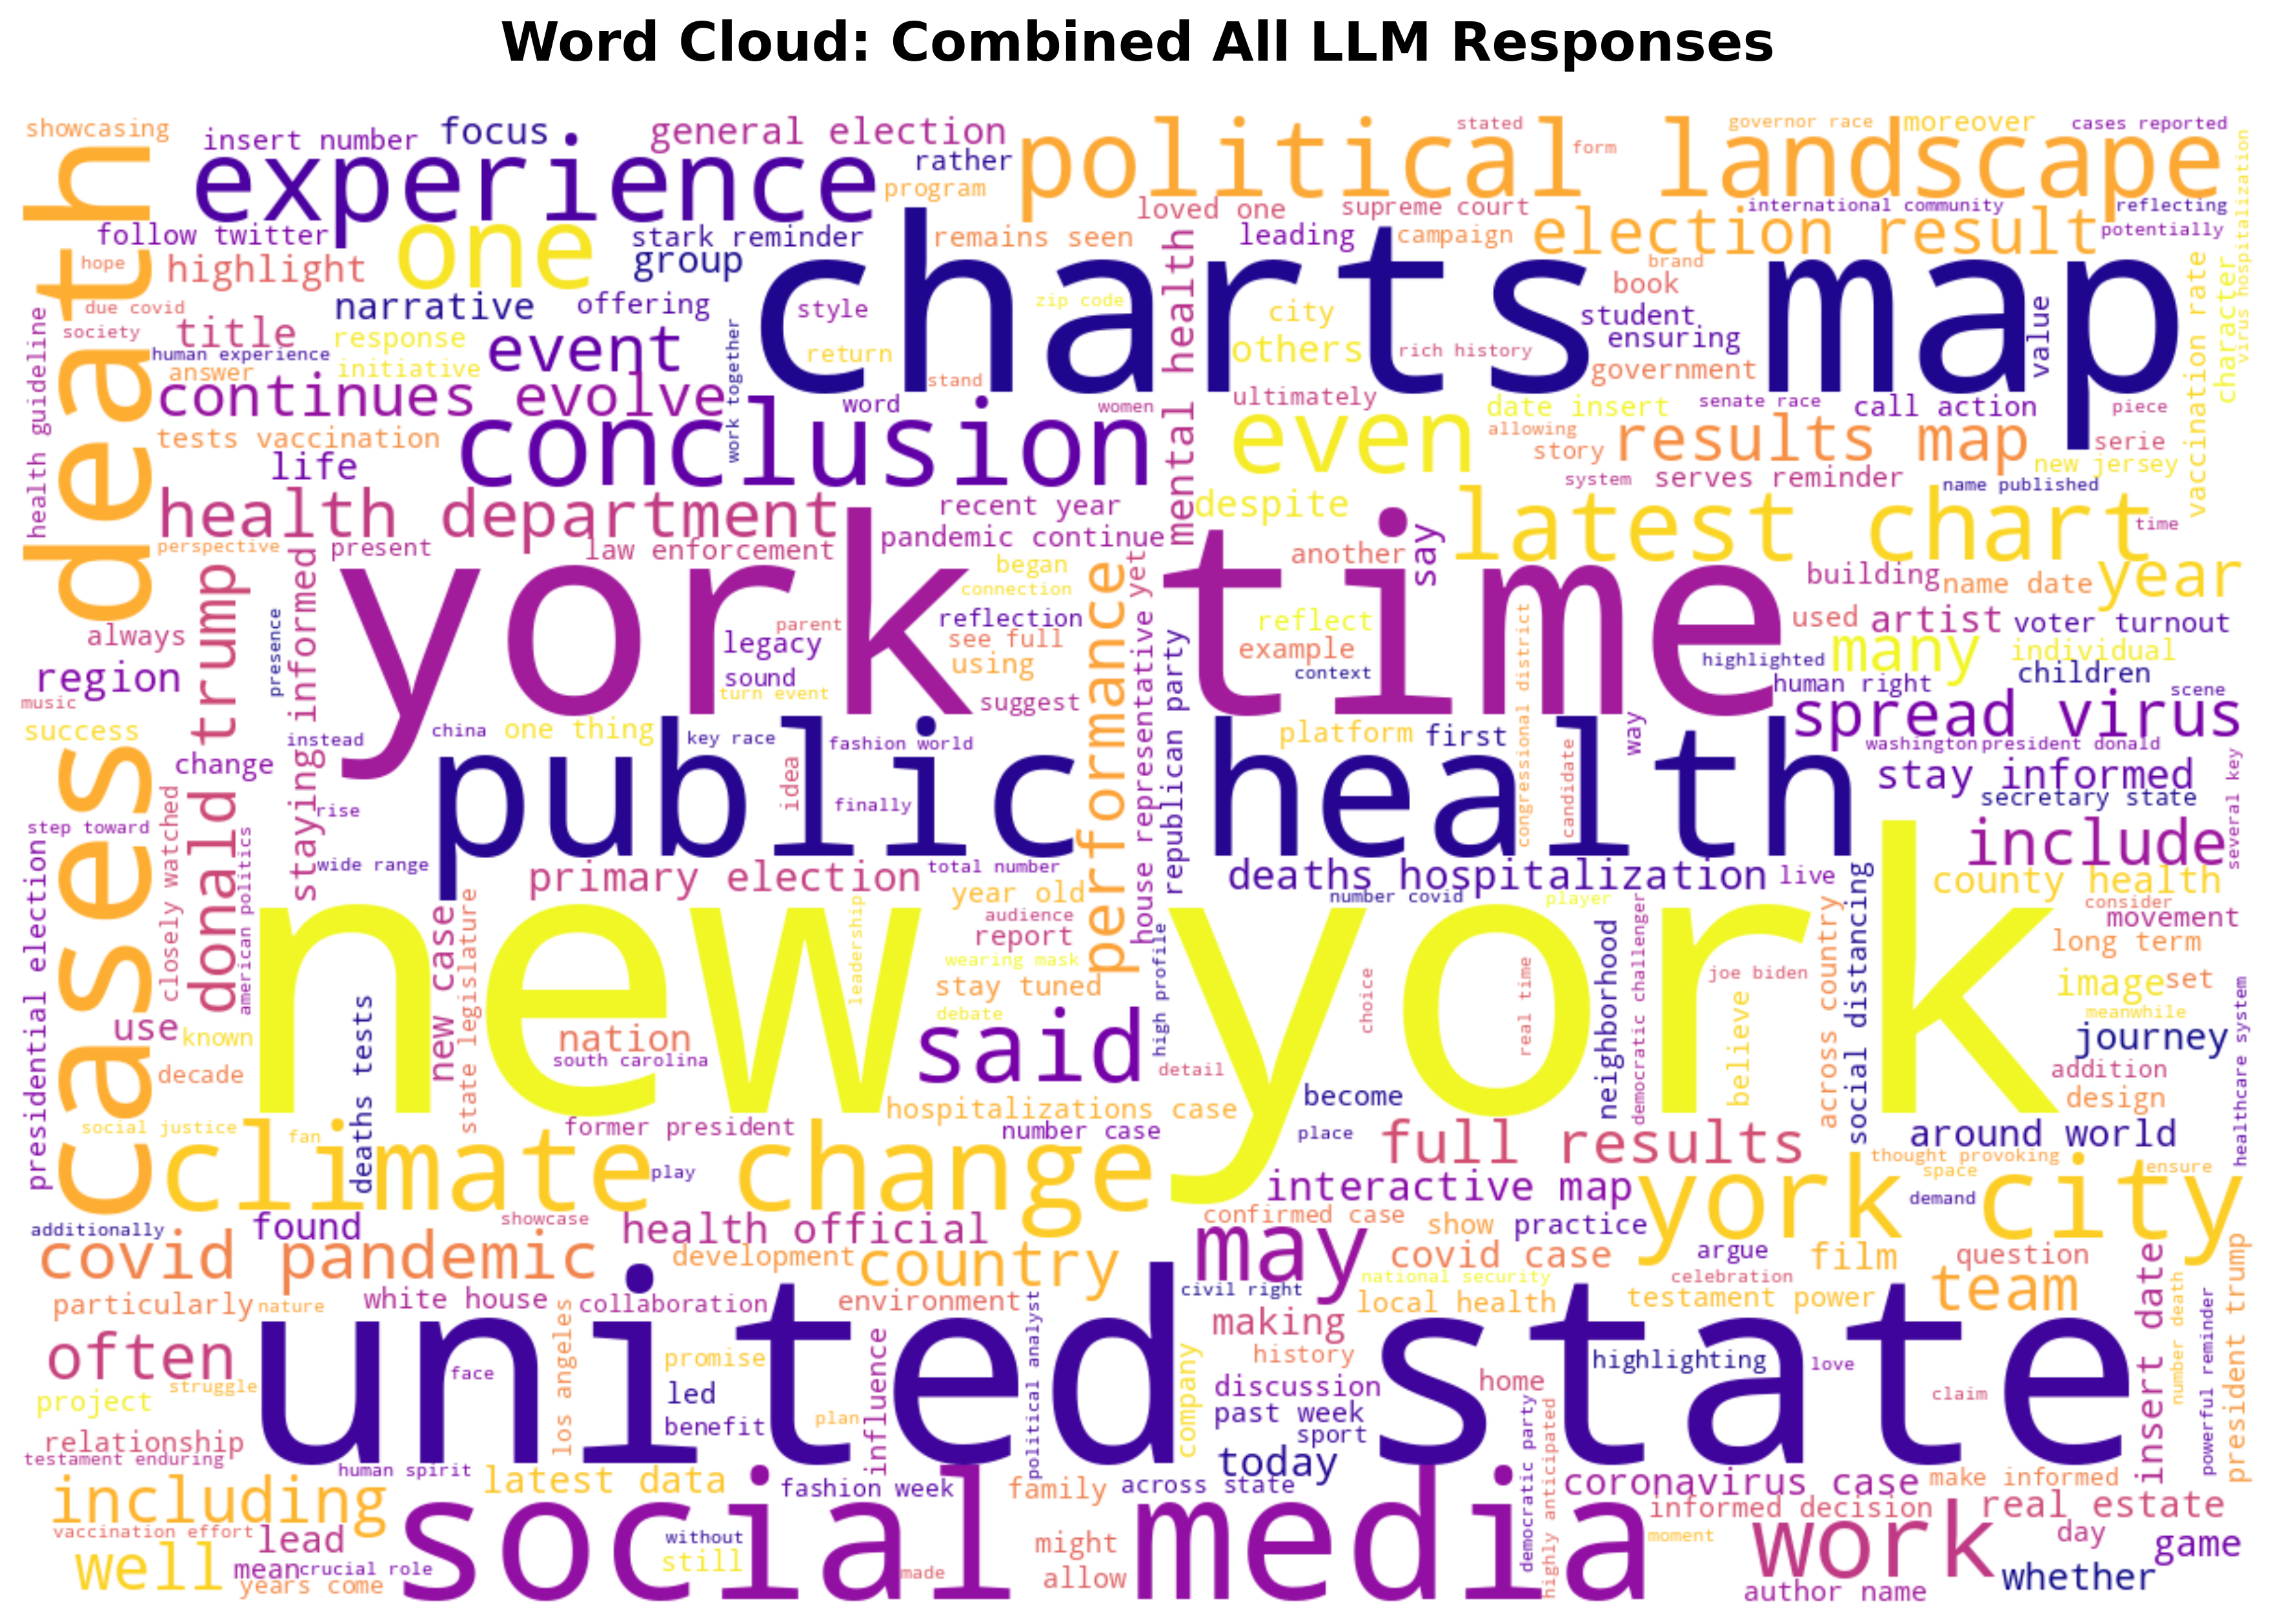
\includegraphics[width=.45\textwidth]{wordcloud_combined_all_llms.png}
    }\hspace{1em}
    \caption{Wordcloud of human written and AI generated text. } 
    \label{fig:wc} 
\end{figure*}

\subsection{base data source}
Our dataset is built upon a large-scale collection of New York Times (NYT) articles spanning January 1, 2000, to the present day. The core NYT dataset comprises over 2.1 million articles and is updated daily, ensuring that the resource remains current and reflective of evolving news trends. Key metadata fields include the abstract of the article, web URL, headline, keywords, publication date, news desk, section name, byline, word count, among other features. These attributes not only capture the diversity of topics covered by the NYT but also provide rich context for further analysis. %Here is the link to our dataset: 



\subsection{Feature Extraction and Transformation}
\paragraph{Abstract as Prompt:} 
The article abstract is extracted and used as a prompt to generate AI text outputs. This serves as a controlled input for language model experiments, ensuring that each generated output is grounded in real-world journalistic content.

\paragraph{Web URL for Human Story Extraction:} 
The provided web URL for each article is utilized to fetch the full human-authored narrative (hereafter referred to as the ``human story''). This extraction captures the in-depth reporting and storytelling inherent to the source material.

\subsection{Generation of AI Texts}
Using the article abstracts as prompts, several state-of-the-art language models were used to generate corresponding texts. The models include Gemma-2-9b, Mistral-7B, Qwen-2-72B, LLaMA-8B, Yi-Large  and GPT\_4-o.

The dataset is thus extended to include both the human-authored text (human story) and AI-generated outputs for direct comparison.

\subsection{Dataset Structure and Statistics}
The final assembled dataset is organized into a tabular format with the following nine columns:
\begin{itemize}
    \item \textbf{Prompt:} The original abstract extracted from the NYT articles.
    \item \textbf{Human\_story:} The full narrative text fetched via the article’s web URL.
    \item \textbf{gemma-2-9b:} AI-generated text produced using the Gemma-2-9b model.
    \item \textbf{mistral-7B:} Output text from the Mistral-7B model.
    \item \textbf{qwen-2-72B:} Text generated by the Qwen-2-72B model.
    \item \textbf{llama-8B:} Output from the LLaMA-8B model.
    \item \textbf{yi-large:} Text generated by the Yi-Large model.
    \item \textbf{gpt\_4-o:} AI-generated output from GPT\_4-o.
\end{itemize}

\begin{table}[h]
\centering
\begin{tabular}{lr}
\hline
\textbf{Column} & \textbf{Count} \\
\hline
Prompt         & 7321 \\
Human\_story   & 7295 \\
Gemma-2-9b     & 7310 \\
Mistral-7B     & 7316 \\
Qwen-2-72B     & 7314 \\
LLaMA-8B       & 7306 \\
Yi-Large       & 7319 \\
GPT\_4-o       & 7321 \\
\hline
\textbf{Total} & 58502 \\
\hline
\end{tabular} 
\caption{Data distribution across real data and varion LLM generated articles. }
\label{tab:aggregated_counts_total}
\end{table}


In total, we have over 58,000 real and synthetic arcitles. The detailed distribution is provided in Table \ref{tab:aggregated_counts_total}. Each LLM contributes roughly equal number of articles.  The dataset is available at:\href{https://huggingface.co/datasets/gsingh1-py/train}{https://huggingface.co/datasets/gsingh1-py/train}.

Figure \ref{fig:wc} shows the wordclouds of human written and AI generated text (combination of all LL generated data) respectively. We can see that key words like "new york", "united state" are prominent across both. 



\subsection{Potential uses of the dataset}
This dataset is uniquely positioned to advance research in the detection of AI-generated content. With a dual composition of human-authored texts (human stories) and AI-generated outputs from multiple state-of-the-art language models, the dataset provides a rich, annotated resource for developing, training, and benchmarking AI content detection systems. Key research directions include:
\begin{itemize}
    \item \textbf{Develop Robust Classifiers:} Create and evaluate models that distinguish between human-written and AI-generated text, improving the transparency and trustworthiness of digital content.
    \item \textbf{Feature Engineering:} Investigate linguistic, stylistic, and semantic features that are indicative of AI generation. This may involve advanced natural language processing techniques and deep learning methods to capture nuanced patterns that differentiate the two text types.
    \item \textbf{Cross-Model Generalization:} Since the dataset includes outputs from multiple language models (e.g., Gemma-2-9b, Mistral-7B, Qwen-2-72B, LLaMA-8B, Yi-Large, GPT\_4-o), it offers a comprehensive basis to study whether detectors trained on one model’s output can generalize to others—a crucial aspect given the rapid evolution of AI text generators.
    \item \textbf{Benchmarking and Model Evaluation:} Benchmark the performance of various AI content detection algorithms by comparing metrics such as precision, recall, and robustness under adversarial conditions.
    \item \textbf{Implications for Misinformation and Authenticity:} In an era where AI-generated text can be misused to spread misinformation or manipulate public opinion, robust detection methods are essential for verifying the authenticity of news content. This dataset supports research that aims to mitigate risks associated with the misuse of AI-generated narratives, reinforcing trust in reputable sources like the New York Times.
    \item \textbf{Hybrid Content Recommendation Systems:} Beyond detection, insights derived from this dataset can inform systems that not only recommend content but also flag or annotate texts based on their origin. This hybrid approach would empower users and platforms to navigate mixed content landscapes more effectively.
\end{itemize}
By combining real-world, human-authored journalism with a spectrum of AI-generated texts, our dataset offers an unprecedented resource for exploring and advancing AI content detection methodologies, ultimately contributing to more secure and transparent information ecosystems.



\subsection{Baseline}

We implement a classification-based baseline inspired by the Raidar method \cite{mao2024raidargenerativeaidetection}, which detects machine-generated content via rewriting. The key idea is that large language models (LLMs) tend to make fewer edits when rewriting content originally generated by another LLM, as opposed to human-written text, which they tend to revise more extensively. This concept can be further extended to hypothesize that an LLM will make even fewer edits when rewriting text originally generated by itself, compared to text generated by a different LLM. This is due to the structural and stylistic consistencies within the outputs of a given LLM, which make its own generations more "acceptable" or lower-loss candidates during rewriting. As a result, measuring the degree of rewriting not only helps distinguish AI-generated from human text, but also allows us to infer the specific model that likely generated the input.

As illustrated in Figure~\ref{fig:baseline_pipeline}, our method prompts a fixed rewriting model (e.g., GPT-3.5-Turbo) with a standardized instruction (e.g., “Concise this for me and keep all the information”) to rewrite the input text. The figure visually demonstrates that human-written inputs typically result in larger modifications during rewriting—highlighted by numerous character-level insertions and deletions—whereas AI-generated inputs lead to much smaller changes, reflecting the model's tendency to preserve its own generative style.

In our classification-based baseline, for each input text, we prompt multiple candidate LLMs (e.g., GPT variants) to rewrite the text and compute the edit distance between their rewritten output and the original input using the Levenshtein metric. The model whose rewrite is closest (i.e., has the minimum edit distance) is predicted as the most likely generator of the input. If all edit distances exceed a predefined threshold—chosen as the \textbf{median} of the \textbf{maximum edit distance} across training samples—the input is classified as human-written. 

\begin{center}
    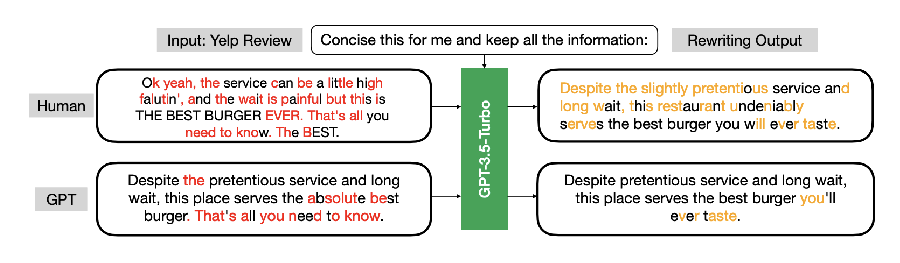
\includegraphics[width=0.9\textwidth]{image/raidar_image.pdf}
    \captionof{figure}{\textbf{Illustration of Raidar concept.} Given a Yelp review, GPT-3.5-Turbo is asked to rewrite the input text while preserving meaning. The rewriting of a human-written review undergoes more character-level edits (highlighted in red/orange), while the rewriting of a GPT-written review remains largely unchanged.}
    \label{fig:baseline_pipeline}
\end{center}

\section{Results}

We define 2 tasks on the dataset: Human vs AI generated text classification (task A) and model attribution for AI-generated text (task B). The results of our baseline on both the tasks are provided in table \ref{tab:result}. These results establish foundational performance metrics for two key classification tasks based on our dataset, and serve as reference points for future research and method development.



\begin{table}[h]
\centering
\begin{tabular}{|l|c|c|}
\hline
\textbf{Task} & \textbf{Description} & \textbf{Accuracy} \\
\hline
Task A & Human vs. AI-generated text classification & 0.5835 \\
\hline
Task B & Model attribution for AI-generated text    & 0.0892 \\
\hline
\end{tabular}
\caption{Results of our baseline. }
\label{tab:result}
\end{table}

For Task A, the baseline uses an edit-distance rewriting approach inspired by Raidar~\cite{mao2024raidargenerativeaidetection} to distinguish human-written from AI-generated texts, achieving an accuracy of 58.35\%. For Task B, the same methodology is employed to identify the originating model of AI-generated texts, yielding an accuracy of 8.92\%.

These baseline scores demonstrate the inherent difficulty of both tasks, especially as modern language models continue to improve. The dataset enables the development and benchmarking of more sophisticated detection and attribution techniques.

\section{Conclusion}
In this paper. We describe and release a comprehensive dataset containing 58k human written and AI generated news samples. Six LLMs are used for AI generated content. We propose two tasks based on the dataset : AI generated text detection and model attribution for AI generated text.  Baseline classification methods give poor results, demonstrating the difficulty of the task and the need for further research.  

Future research could include expanding the dataset to other languages and modalities. More sophisticated methods to detect AI generated text is also an interesting line of future work. 

% \printbibliography
% \bibliographystyle{plainnat} % or another style like abbrvnat, unsrtnat
\bibliography{references} % Ensure you have a references.bib file
\end{document}